\chapter{Der Segelflugrechner}\label{cha:glide}
In diesem Kapitel wird beschrieben, wie das Programm intern arbeitet und es ist wirklich empfohlen,
sich hiermit zu beschäftigen. Nur dann können einige der Anzeigen bzw.\ Berechnungen von textsf{XCSoar's}
wirklich richtig gedeutet werden.
Ein Mindestmaß an Überlandflugerfahrung  wird voraus gesetzt, insbesondere sollte die MC-Theorie
halbwegs verstanden sein.

Dennoch ist es problemlos möglich mit dem Programm 'durch die Gegend' zu fliegen und sich von ihm in
vielen Dingen unterstützen zu lassen.

\section{Die verschiedenen Flugmodi}\index{Flugmodi!Unterschiede}
Je nach Flugmodus berechnet \textsf{XCSoar} die Daten teils unterschiedlich und gibt diese in frei
definierbaren Datenfenstern, den sog.\ Infoboxen wieder. Als Flugmodus werden hier Kurbeln (thermalling),
einfacher Vorflug (cruise) oder Endanflug (final glide), einer besondern Art des Vorfluges,
nämlich auf den letzten Wegpunkt also den Zielpunkt einer Aufgabe hin,  unterschieden.

\textsf{XCSoar} kann automatisch zwischen Kurbel-  und Vorflugmodus unterscheiden. Die Umschaltung
der verschiedenen Berechnungsmethoden hierbei geschieht automatisch.  Nach ca.\ 30 Sekunden Kurbelzeit
schaltet die Software automatisch auf den Kurbelmodus. Nach 30 Sekunden Geradeausflug schaltet das
Programm auf den Vorflugmodus. Es besteht auch die Möglichkeit diese Umschaltung manuell über das Menü zu erzwingen.

Ist der letzte Wegpunkt (Zielpunkt) aktiv, wird in den Endanflugmodus geschaltet.
Der Endanflugmodus wird ebenfalls aktiviert, wenn eine Aufgabe abgebrochen wird, so daß hier immer
auf die erreichbaren Punkt gerechnet wird.

Ein kleines Symbol in der rechten unteren Ecke zeigt den jeweiligen Flugmodus an:
\begin{center}
\begin{tabular}{c c c c}%{c c c c}

\includegraphics[angle=0,width=0.75cm,keepaspectratio='true']{icons/mode_cruise.pdf} &

\includegraphics[angle=0,width=0.75cm,keepaspectratio='true']{icons/mode_climb.pdf} &

\includegraphics[angle=0,width=0.75cm,keepaspectratio='true']{icons/mode_finalglide.pdf} &

\includegraphics[angle=0,width=0.75cm,keepaspectratio='true']{icons/mode_abort.pdf}\\
(a) & (b) & (c) & (d)
\end{tabular}
\end{center}

\begin{description}
\item[\textit{Vorflug}  (a)]   Das Flugzeug ist nicht am Kurbeln  und es ist entweder keine Aufgabe aktiv, oder
der aktive Wegpunkt ist nicht der Aufgaben-Zielpunkt
\item[\textit{Kurbeln} (b)]  Das Flugzeug ist derzeit am Kurbeln (auch wenn es dabei nicht steigt oder gar sinkt!)
\item[\textit{Endanflug} (c)]  Das Flugzeug ist nicht am Kurbeln und der aktive Wegpunkt ist der Zielpunkt der Aufgabe.
\item[\textit{Abbruch} (d)]  Dieser manuelle Aufgabenabbruch zeigt an, daß sich das Programm in einem  Modus befindet, in dem ausschließlich Außenlandemöglichkeiten auf landbaren Plätzen, Flugplätzen und markierten Feldern  dargestellt und berechnet werden, die sich in den entsprechenden Datenbanken befinden.. 
(siehe Kap.~\ref{sec:abort-resume-task})
\end{description}

Die jeweiligen Berechnungen von \textsf{XCSoar} sind direkt abhängig vom jeweiligen Flugmodus. Die
Anzeige der Daten, insbesondere die der Infoboxen wechseln komplett und frei definierbar von Modus zu
Modus. Auch der Zoom-Modus kann beim Umschalten der Modi automatisch geändert werden.

Zusätzlich zu diesen Anzeige-Modi können mehrere Sätze an Infoboxen frei benannt und belegt werden,
welche während des Fluges unabhängig vom jeweiligen Flugmodus aufgerufen werden können.

Der Endanflugmodus ersetzt den normalen Vorflugmodus sobald der Flieger oberhalb der notwendigen
Endanflughöhe ist. Die hierzu benötigte Höhe ist maßgeblich abhängig vom eingestellten MC-Wert, aber
auch die Höhe über Grund und Sicherheitshöhen werden berücksichtigt.

Wird während eines Endanfluges mit dem Kurbeln begonnen, wird\textsf{XCSoar} in den Kurbelmodus umschalten und
sobald der Endanflug wieder fortgeführt wird, zurück in den Endanflug-Modus geschaltet.

\section{MacCready setting}

Der  MacCready Wert kann auf verschiedene Weisen eingegeben werden:
\begin{itemize}
\item Von den Menupunkten
\begin{quote}
\bmenu{Konfig.}\blink\bmenu{MC $+$}

\bmenu{Konfig.}\blink\bmenu{MC $-$}
\end{quote}
\item Bei  Touchscreen-Geräten (Android, PDA), kann auch die entsprechende Infobox direkt angewählt
werden und mit den Hoch/Runter Knöpfen (Android) bzw. der Schaltwippe (PDA)der Wert geändert werden.
\item Ist \textsf{XCSoar} an ein intelligentes Vario wie z.B.\ das Vega angeschlossen, dann
ändert die MC Einstellung im Vario auch die in \textsf{XCSoar}.
\end{itemize}

Als zusätzliche Option ist ein Automatik-MC-Mode verfügbar und in Kap. ~\ref{sec:auto-maccready} beschrieben.

\section{Flugzeugpolare}

Eine große Anzahl an Polaren ist in \textsf{XCSoar} bereits vorhanden und kann
somit sofort  ausgewählt werden. Wenn ein Flugzeugtyp nicht vorhanden sein
sollte, so können z.B. Näherungswerte der vorhanden  Flugzeuge benutzt werden.

In diesem Falle ist es ratsam, sich an den im Internet auf bekannten Seiten
vorhandenen Polaren zu beschaffen und entsprechend anzupassen. Siehe hierzu
auch \config{polar}.

Die Polare kann während des Fluges angepaßt werden, um z.B. Mückenbefall einzustellen
und so die Gleitleistung entsprechend zu verschlechtern oder aber entsprechend Wasserballast entsprechend zu verbessern.

Wie bekannt und von jederman sicher schon leidvoll erfahren, bewirkt
Mückenbefall und/oder  Regen eine teils drastische  Verschlechterung der
Gleitleistung des Flugzeuges. Bislang sind Rechner bzw. Programme noch nicht in
der Lage, diese automatisch zu erkennen, sodaß es allein in der Macht und
Erfahrung des Piloten liegt, eine Einschätzung der Verschlechterung vorzunehmen
und diese als Parameter (in Form eines Prozentwertes) dem Programm mitzuteilen.

Hierbei entsprechen 100\% Mücken Faktor einem sauberen Profil (linke Seite), 50\% bedeuten eine Verdopplung der
Sinkrate des Flugzeuges - verglichen mit dem sauberen Profil.

\begin{center}
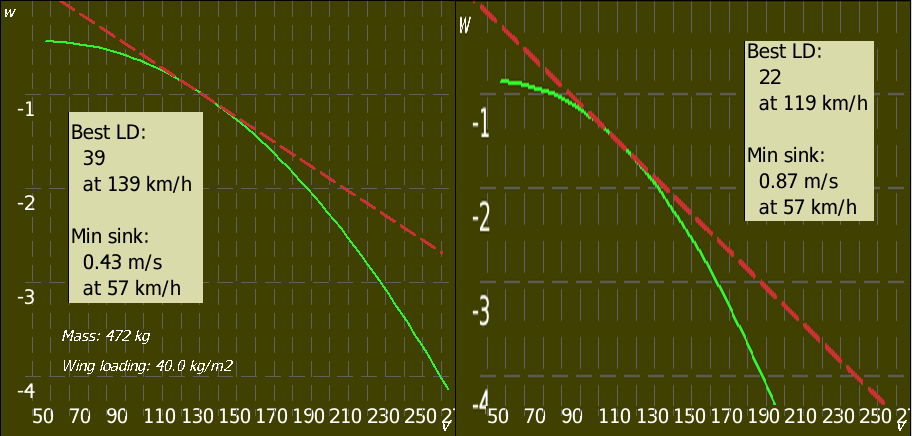
\includegraphics[angle=0,width=\linewidth,keepaspectratio='true']{figures/cut-clean-dirty-polar.png}
\end{center}

Es ist bekannt, daß Mückenbelastung die Flugleistungen eklatant verschlechtern können, mir ist ein Fall bekannt, in dem die
Verschmutzung so drastisch war, daß sogar eine bekanntermaßen "harmlose" ASK21 bei der Landung einfach durchsackte und
dem Piloten einige Wochen im Krankenhaus verschaffte\dots Ein anderer Pilot berichtete während es gleichen Fluges davon, daß seine
Mückenputzer nicht ausgefahren werden konnten, da diese an den Massen der Läuse hängen blieben\dots

Dies alles vorausgesetzt, ergeben sich praktisch resultierende Verschlechterungen der Gleitleistung und somit Verschiebung
der Polare der Polare für den "worst case" von 30 - 70\%.

Es sind sicherlich einige "Probeflüge" notwendig, um die entsprechende Verschlechterung durch Mückenbelastung einschätzen
und entsprechend al Prozentangabe in den Rechner eingeben zu können, die vor allem vor dem Hintergrund,
daß alle Flugzeugprofile sich hierin unterscheiden.

Der Wert für den Ballast  wird in \xc eingestellt als eine prozentuale Einstellung des \textsl{maximal möglichen Ballastes}.
\index{Ballast-Einstellung}\index{Wasserballast-Einstellung}
Abhängig von der Konstruktion des Segelflugzeuges bzw.\ insbesondere seiner Polaren kann diese Einstellung  durch das
jeweilige Gewicht des Piloten in großem Rahmen variieren.

So kann z.B. wenn ohne Wasserballast geflogen wird, die Einstellung dennoch auf z.B.\ 10\% eingestellt werden,
um dem wahren Abfluggewicht des Flugzeuges näher zu kommen.


%{\it DIAGRAM SHOWING GLIDE POLAR, 0\% BALLAST AND 100\% BALLAST}

Die zur Berechnung herangezogene Polare und das eingegebene Gesamtgewicht kann
u.a. im Analyse-Dialog betrachtet werden, welches hier später behandelt wird.

\section{Flug Einstellungen (dialog)}\label{sec:basic-sett-dial}
In diesem Menü können die folgenden Einstellungen vorgenommen werden:


\menulabel{\bmenut{Konfig.}{1/2}\blink\bmenut{Flug}{Einstellungen}}
\begin{itemize}
\item Wasserballast
\item Flächenbelastung
\item Insekten (Mückenbelastung)
\item QNH
\item Max. Temperatur
\end{itemize}

Mithilfe der Mückeneinstellung kann während des Fluges \achtung nachjustiert werden, wie sich die Polare
durch Mückenbefall verschlechtert.  0\% bedeutet, daß die Software annimmt, das Flugzeug bzw.\ 
das Profil ist top sauber. 

Eine Einstellung von 50\%  wird die Polare um 50\% verschlechtern, was in etwa der Verdopplung
der Sinkrate bei der entsprechenden Geschwindigkeit entspricht.

\sketch{figures/dialog-basicsettings.png} Die Ballast Einstellungen werden benutzt, um  die Polare entsprechend der Flächenbelastung verschieben zu können. Der Ballast wird in Litern angegeben, und sollte \emph{vor} dem Flug
korrekt angegeben werden.


Dieser Dialog kann vor und während des Fluges benutzt werden, um das QNH einzustellen.
Die Software benutzt diese Werte um während des Fluges die entsprechenden Flugflächen
zu errechnen. Wenn mit einem intelligenten unterstützten Vario bzw. Höhenmesser verbunden,
kann wird die Höhe in diesem Dialog eingestellt werden. Das macht es sehr einfach,
das QNH einzustellen, wenn die Höhe des Flugplatzes bekannt ist.


Die maximale vorhergesagte Boden-Temperatur kann hier eingegeben werden und wird dann für die
Konvektionsvorhersagen verwendet. (siehe Abschnitt~\ref{sec:convection-forecast})
Hieraus werden dann Höhe der Konvektionsschicht und Basis der Wolken ermittelt.


Beim Systemstrat wird, nachdem ein GPS als solches erkannt ist und über einen Drucksensor verfügt,
das QNH automatisch ermittelt.  Diese Korrektur setzt das QNH so, daß die Druckhöhe mit der
Geländehöhe übereinstimmt.

Das QNH wird nur dann aktualisiert, wenn das Flugzeug für mehr als 10 Sekunden auf dem Boden
steht! (um den Abgleich mit der Geländedatei zu ermöglichen.)

Sollte \textsf{XCSoar} im Fluge neu gestartet werden, so ist das QNH nicht mehr aktuell! \index{QNH!Ermittlung!Korrektur}
Die Aktualisierung kann weiterhin ausschließlich dann erfolgen, wenn Geländedatei aktuell und in
Ordnung ist - darin sind ja die Geländehöhen MSL enthalten...

\section{Sollfahrt}\index{Sollfahrt}

Wenn das Programm mit einem intelligenten Vario betrieben wird, welches die angezeigte
Fluggeschwindigkeit (IAS) berechnet, dann werden am rechten Rand der Anzeige Geschwindigkeitspfeile
angezeigt. Wenn das Flugzeug schneller als die optimale Geschwindigkeit fliegt, dann zeigen grüne Pfeile
nach oben (ziehen !), wird zu langsam geflogen, zeigen rote Pfeile nach unten. Wird mit optimaler
Geschwindigkeit geflogen, so erscheinen keinerlei Pfeile.

%{\it DIAGRAM SHOWING SPEED COMMAND CHEVRONS}

Abhängig von der jeweiligen Konfiguration erscheinen die Geschwindigkeitspfeile entweder
am rechten Rande des Bildschirmes oder aber in der Vario-Anzeige.

\section{Sollfahrt - Empfohlene Geschwindigkeit}\index{Sollfahrt!MC oder Delphinstil}

\textsf{XCSoar} berechnet kontinuierlich zwei Sollfahrten gemäß der Polare des Flugzeuges und der
MC-Theorie:

\begin{description}
\item[\textit{MacCready Geschwindigkeit}]  Diese Geschwindigkeit ist die optimale Vorfluggeschwindigkeit nach der
MC Theorie in ruhender Luft, unter Berücksichtigung des Windes, wenn im Endanflug.
\item[\textit{Delphin-Stil- Geschwindigkeit}]  Dies ist die optimale Vorfluggeschwindigkeit unter
    Berücksichtigung von aufsteigender und fallender Luft sowie unter Berücksichtigung des Windes,
    wenn im Endanflug.
\end{description}

Diese Geschwindigkeiten haben nichts mit der Geschwindigkeit beim Kurbeln zu tun!
Der Pilot kann diemaximal zulässige Manövergeschwindigkeit im Konfigurationsbereich
eingeben, welche die empfohlenen Geschwindigkeiten anhand der MC-Werte in einen
realistischen Bereich eingrenzen.

Je nach Pilot gibt es verschiedene Vorlieben:

manche bevorzugen dies sogenannte "block-speed", d.h., sie fliegen zwischen zwei Bärten mit konstanter
Geschwindigkeit\index{Block-Speed}, streng nach der MC-Theorie; andere dagegen
variieren auch zwischen zwei Bärten, gemäß des "Delphin"-Flugstieles\index{Deplhin-Stil}, wobei die
Geschwindigkeit permanent angepasst wird.


\begin{maxipage}
\begin{center}
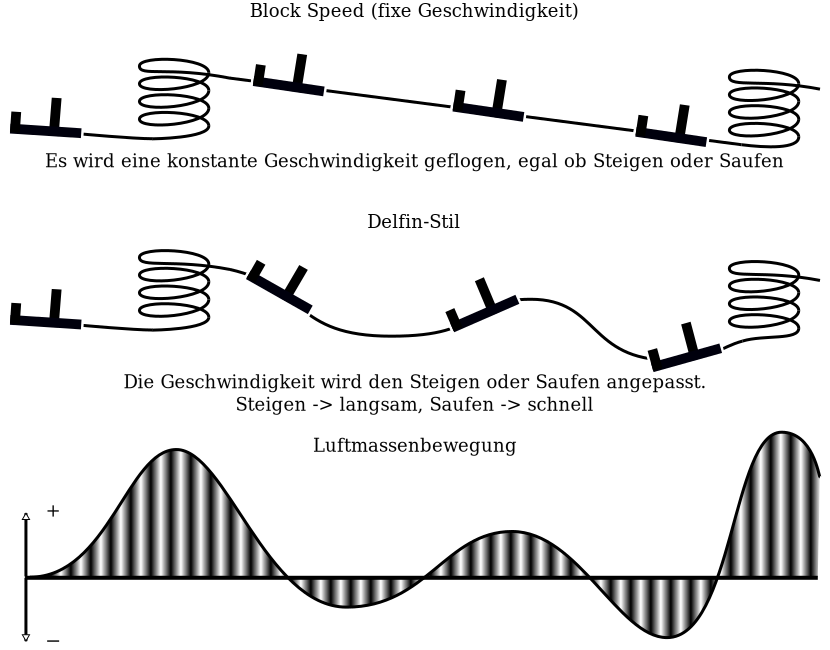
\includegraphics[angle=0,width=0.8\linewidth,keepaspectratio='true']{figures/figure_speed_to_fly-de.pdf}
\end{center}
\end{maxipage}

In der Konfigurationseinstellung "Block-Speed-to-fly" (~\ref{sec:final-glide})
kann eingestellt werden, ob der Delphinstil, oder der "pure" MC-Wert zur
Berechnung herangezogen werden soll.

Die \infobox{V opt} zeigt ebendiese Geschwindigkeit, je nach
ausgewählter Methode an.\index{Sollfahrt!InfoBox}

Falls an das VEGA Vario angeschlossen, werden die Töne des Varios im Sollfahrt-Modus
genau anhand dieses Wertes ausgegeben.


\section{Sollfahrt  mit Risikofaktor}\label{sec:speed-fly-with}\index{Sollfahrt!Risikofaktor}
Viele Piloten verringern den MC-Wert und somit die Sollfahrt wenn Sie während der Aufgabe niedriger werden.
 Die interne Sollfahrtberechnung kann mit einem Risikofaktor belegt werden, welcher je nach erreichter Flughöhe in beiden Fällen
 (Delphin oder Block-Speed) den MC Wert automatisch verringert, je mehr man sich dem Boden nähert.

Die Theorie hierfür ist grob geschrieben in einem Aufsatz von John
  Cochrane, ``MacCready Theory with Uncertain Lift and Limited
  Altitude'' {\em Technical Soaring} 23 (3) (July 1999) 88-96.
  \url{http://faculty.chicagogsb.edu/john.cochrane/research/Papers/newmcred.pdf}

Ein konfigurierbarer Parameter, $\gamma$ (`der STF Risiko Faktor '\footnote{STF  = Speed To Fly $\Rightarrow$  Sollfahrt},
in den Konfigurationseinstellungen auf der Seite "Endanflugrechner") erlaubt die Kontrolle, wie der Risiko-MC-Wert berechnet wird.

Der $\gamma$ Faktor bestimmt die Beziehung aus dem aktuell eingestellten MC-Wert als Funktion der Höhenbeziehung.
Der Höhenbeziehung ist bestimmt als das Verhältnis zwischen aktueller Höhe über Grund ($h$) und Basishöhe über Grund ($h_{top}$).

Somit bestimmt $\gamma$ einen Faktor, bestehend aus maximal zu erreichbaren Höhe (Basis minus Geländehöhe)
und der Höhe, bei der man beginnt, über eine evtl. Außenlandung bzw. Abbruch der Aufgabe nachzudenken.

Demgemäß bewirkt ein niedriger Faktor $\gamma$ eine höhere Außenlandetoleranz gegenüber größeren Werten von $\gamma$. Der als Default
gesetzte Wert v0n $\gamma=0$ bewirkt keinerlei  Anpassung, der Risiko MC-Wert ist identisch dem eingedrehten MC-Wert.

Für $\gamma=1$ wird der Risiko-MC-Wert linear mit $h/h_{top}$ angepasst.
Alle Werte dazwischen werden leicht variiert angepaßt, sodaß der der Risisko-MC nur dann auch klein wird, wenn man wirklich niedrig ist.

Kleine Werte von $\gamma$ werden bevorzugt, wenn die Piloten mit geringer werdenden Höhe nicht langsamer werden möchten und so ein
Außenlanderisiko bewußt in Kauf nehmen, höhere Werte von $\gamma$ werden von vorsichtigen Piloten bevorzugt,
resultierten jedoch (aufgrund niedrigerer MC-Werte) in einer niedrigeren Schnittgeschwindigkeit.

Ein Wert von  $\gamma=0.3$ ist empfohlen.

\begin{center}
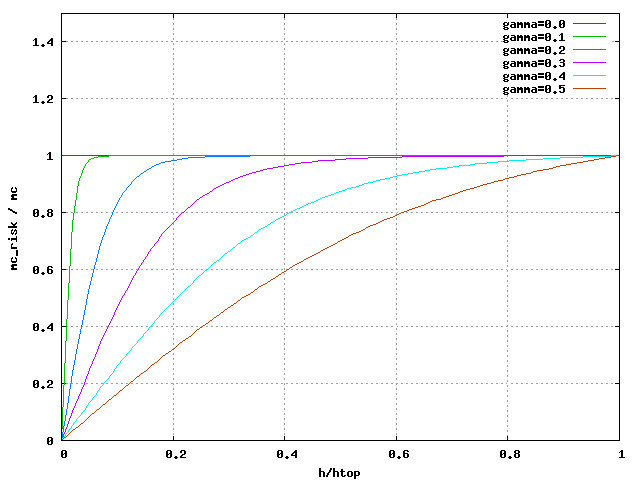
\includegraphics[angle=0,width=\linewidth,keepaspectratio='true']{figures/riskmc.png}
\end{center}

\section{Sicherheitshöhen}\label{sec:safety-heights}\index{Sicherheitshöhe!Spezielle}

In \xc werden drei Sicherheitshöhen deklariert und benutzt, welche ein abgestuftes Maß von Sicherheit in die Berechnungen einfließen lassen.

Die Sicherheitshöhen sind:
\begin{description}
\item[\textit{Ankunftshöhe}]
Dies ist die Ankunftshöhe über Grund über dem aktiven Wegpunkt, bei welchem das Flugzeug  eine sichere Platzrunde
zur Landung erreichen wird, zusätzlich einer gewissen Reserve.

Dieser Wert wird im Endanflug benutzt und ist bestimmend für die Anzeige und das Erreichen von alternativen landbaren Feldern.


\item[\textit{Überlandfreiheit "Terrain  clearance"}]
Dies ist die Höhe über Grund, unterhalb derer jeder berechnete Gleitpfad zu nicht
angepassten Höhen des Weiterfluges führen wird.

Die Überlandfreiheit beeinflußt die Reichweitenanzeige  und, falls der Endanflug zu irgendeinem
Punkt unterhalb der Höhe über Grund führen sollte, erscheint ein rotes Kreuz als Zeichen für den "Aufschlagpunkt".

Sollte das Geländemodell ungültig sein oder außerhalb der Reichweite, dann wird dies Geländewarnmerkmal deaktiviert.

\item[\textit{Aufbruchshöhe "Break-off height"}]
Dies ist die Höhe über Grund, bei der sich der Pilot Gedanken machen sollte, den Überlandflug abzubrechen
bzw.\ sich mit einen Außenlandeacker beschäftigen sollte.

Derzeit wird diese Höhe noch nicht innerhalb der Berechnungen benutzt, aber für spätere Zwecke schon eingeführt.
\end{description}

\begin{maxipage}
\begin{center}
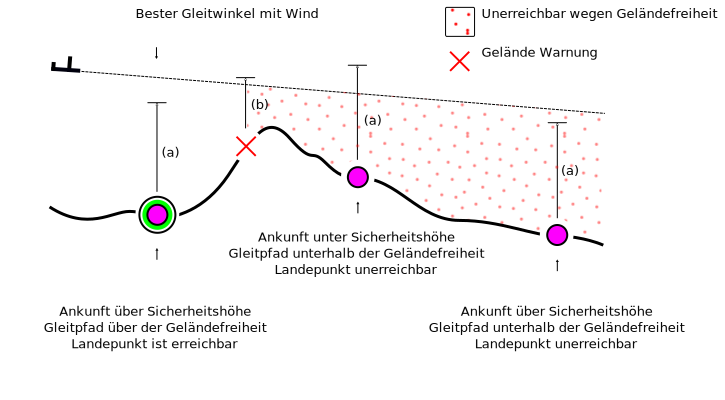
\includegraphics[angle=0,width=\linewidth,keepaspectratio='true']{figures/figure_terrain-de.pdf}
\end{center}
\end{maxipage}

\warning
Diese Höhen können auf  Null gesetzt werden, es ist jedoch grundsätzlich empfohlen, mit einer gewissen Reserve als Sicherheit
zu fliegen, da kein bisher auf dem Markt verfügbarer Rechner oder aber Software in die Zukunft bzw.\  in das Wetter schauen kann.
(Ich denke mal, das wird auf absehbare Zeit auch so bleiben -\textsf{OH})

\textsf{XCSoar} benutzt zur Berechnung der Ankunftshöhen die MSL eines jeden Punktes aus dem Wegpunkt-File, oder aber,
falls hierin nichts eindeutiges drin vermerkt ist, die Daten aus dem Höhenmodell des Kartenmaterials (also des XCM-Files)

\textbf{Die angezeigte Ankunftshöhe  des nächstliegenden, landbaren ausgewählten Wegpunkte werden standardmäßig
mit MC=0  und mit dem besten Gleiten aus der eingestellten Polare errechnet, der Wind wird hierbei mit berücksichtigt.
\warning Ein Sicherheits-MC-Wert kann und sollte bestimmt und in den Konfigurationseinstellungen eingestellt werden, wie im Kapitel
oben beschrieben.}



Landbare Felder werden nur als erreichbar angezeigt, wenn die Ankunftshöhe oberhalb  der Ankunftssicherheitshöhe liegt und der
Gleitpfad zu keinem Punkt durch Geländeerhöhungen bzw. der Überlandfreiheit (s.o.) begrenzt beschränkt ist.


Wenn der Endanflug durchs Gelände führen würde, ist, Wolkenstraßen oder Hangwind o.ä. ausgenommen,
ziemlich sicher, daß erneut gekurbelt werden muß, um sicher (also mit den eingestellten Werten) den
Wegpunkt erreichen zu können.

Während der Berechnung der Ankunftshöhen aller landbaren Felder/Plätze kann ein ebenfalls
Sicherheits-MC- Wert eingestellt werden. Dieser Wert ist standardmäßig auf Null gesetzt.

Größere Werte führen zu konservativeren (sichereren) Anflügen.

\section{Endanflugrechner}\index{Endanflugrechner}

Der Endanflugrechnern benutzt mannigfaltige Informationen und Quellen um die Ankunftshöhe und Zeit zu berechnen.
Diese sind im einzelnen:

\begin{itemize}
\item Die Flugzeugpolare.
\item Windrichtung und -geschwindigkeit
\item Entfernung und Kurs zum Zielpunkt
\item MC-Wert
\item Höhe des Zielpunktes
\item Benutzerdefinierte Sicherheitshöhen
\item Die Totalenergie des Flugzeuges, falls das Flugzeug mit einem enstprechenden Gerät ausgestattet, dies mit \xc
verbunden ist und die IAS angibt.
\end{itemize}

Aus den oben genannten Parametern, können zwei Höhen errechnet werden:

\begin{description}
\item[\textit{Benötigte Höhe}]
Diese Berechnung gibt die insgesamt benötigte Höhe um das ausgewählte Ziel zu erreichen,
zusätzlich vom Piloten bestimmter Sicherheitshöhen.
\item[\textit{Höhendifferenz}]
Diese Kalkulation errechnet die benötigte Höhendifferenz zum Zielpunkt  plus der Höhe des
Ziels (MSL) minus der Flughöhe des Flugzeuges (MSL).

Das Ergebnis entspricht also entweder der aktuellen Flughöhe über dem Gleitpfad oder aber der Ankunftshöhe am Ziel.
Wenn keine Höhe des Wegpunktes in der Wegpunkt-Datenbank (z.B. \texttt{GER-WP.txt}) hinterlegt ist, wird \textsf{XCSoar}
die Höhe des Geländes aus dem Gelände File (z.B.: \texttt{GER-High.xcm}) benutzen.
%\todonum{und wenn nicht vorhanden? Gibt es eine Fehlermeldung?}
\end{description}

Die Berechnung des Endanfluges ist soweit fortgeführt worden, daß sowohl die Höhen als auch die Höhendifferenzen
berechnet werden, um die komplette Aufgabe zu erfüllen. Auch \textsf{XCSoar} kann also "um die Ecke rechnen"

\tip Diese Höhendifferenz wird permanent am linken Rand des Displays sowohl numerisch als auch als roter,
grüne oder orangene  Pfeile nach unten oder oben dargestellt.\index{Höhe!Benötigt für Aufgabe}\index{Höhe!Anzeigepfeile}

Diese Höhe ist korrigiert um die Energie-Höhe (potentielle Energie), aufgrund der Tatsache, daß potentielle
Energie in kinetische Energie umgewandelt werden kann - abzüglich Verlusten.

Die kinetische Energie, welche vom Flugzeug in Höhe umgewandelt werden kann (Hochziehen) wird aus der
Differenz der TAS zur Geschwindigkeit des besten Gleitens gebildet. Diese Berechnung ist am genausten wenn
entsprechende Daten vorhanden sind (Abgriff vom Fahrtenmesser o.ä.), andernfalls wird die True Airspeed
aus der Wind- und Übergrundgeschwindigkeit ermittelt. Dazu mehr im folgenden Teil

\section{Anzeige der benötigten Höhe für die ganze Aufgabe}\index{Benötigte Höhe für ganze Aufgabe}\index{Endanflugspfeile}

Auf der linken Seite der Karte wird über die gesamte Flugdauer hinweg die für die gesamte Aufgabe benötigte
Höhe sowohl als Pfeil als auch in numerischer Form dargestellt.  Wenn der Flieger oberhalb der minimal erforderlichen Höhe \emph{zum Erreichen der Aufgabe} ist, erscheint ein grüner, nach oben gerichteter Pfeil.
 
Ist der Flieger zu tief, erfolgt die Anzeige ganz ähnlich, aber in rot und nach unten.

Bei mehr als 500m positiver oder negativer Höhe wird zusätzlich eine abgesetzte Pfeilspitze in entsprechender
Farbe dargestellt; dies dient lediglich der augenblicklichen Erkennung der Lage.

\textcolor{blue}{Sollte mit der vorhandenen Höhe \textbf{Landepunkte} \footnote{Achtung!  Das hängt natürlich  davon ab, was in der Datenbank zu den jeweiligen Punkten vermerkt ist!  Ein See, der als landbar markiert ist\dots  tja, da kann man dann auch nix mehr  machen\dots} in Reichweite sein, \achtung die aktuelle Höhe jedoch nicht ausreichen, um die \textbf{ Aufgabe} zu beenden, so werden die Pfeile \textcolor{orange}{orange} angezeigt.}

Wenn man also orange Pfeile sieht, kann man ziemlich sicher sein, daß zumindest ein Landeplatz erreichbar ist, wenngleich die Aufgabe nicht beendet werden kann. 

\begin{center}
\begin{tabular}{c c}
{\it Oberhalb}\phantom{ABC} & \phantom{ABC}{\it Unterhalb} \quad  \\
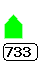
\includegraphics[angle=0,keepaspectratio='true']{figures/cut-fg-above.png} &
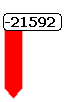
\includegraphics[angle=0,keepaspectratio='true']{figures/cut-fg-below.png}
\end{tabular}
\end{center}
Die Skalierung dieser Pfeile der Endanflugsanzeige beträgt $+/-$ 500 m.  
Die hellere Hälfte des Pfeils (hier nur rechts) steht für MC=0.


\subsection*{Anzeige der benötigten Endanflugshöhe auf dem Bildschirm}\index{Endanflug, benötigte Höhe, Anzeige}\label{sec:finalheight-indicator}

Die Anzeige der benötigten Endanflugshöhe wurde derart gestaltet, daß auf einen Blick der
Einfluß des MC-Wertes sehr übersichtlich erkenntlich wird.

\emph{Die vertikalen Pfeile zeigen die notwendige Höhe zum Beenden der Aufgabe
beim jeweils gewählten MC-Wert und gleichzeitig  bei MC$=0$ an.}

Hierzu sind die Pfeile in den Farben grün, rot und orange dargestellt und zusätzlich ist eine entsprechend
abgesetzte gefärbte Pfeilspitze dargestellt, die ab einer zusätzlich notwenigen oder verfügbaren Höhe
von 500m erscheint.

Halbtransparente Pfeile der gleichen Farbe und halben Breite am linken Rand des Displays geben den entsprechenden Wert für MC$=0$ an.

Die eingeblendete Zahl neben den Pfeilen gibt die notwendige Höhe für den aktuell gewählten  MC-Wert an.

Hier ein paar Beispiele für verschiedene Szenarien:

\begin{description}
\item[\textit{Über Endanflughöhe}] bei  MC$=M$ und MC$=0$:

\marginpar{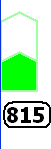
\includegraphics[angle=0,width=2.55em,keepaspectratio='true']{figures/fig-finalglide-allabove.png}}
Bei der derzeitigen MC Einstellung beträgt die Reserve $152m$ wird auf MC$=0$ umgeschaltet gibt es etwas mehr Reserve.
%\marginpar{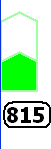
\includegraphics[angle=0,width=1.0cm,keepaspectratio='true']{figures/fig-finalglide-allabove.png}}


\item[\textit{Über Endanflughöhe}] bei MC$=0$ aber unter Endanflughöhe bei  MC$=M$, und :

Hier zeigt  das Display eine Situation, bei der die vorhande Höhe  mit dem eingestellten MC-Wert nicht ausreicht,
\marginpar{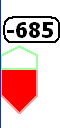
\includegraphics[angle=0,width=3em,keepaspectratio='true']{figures/fig-finalglide-halfabove.png}}um die Aufgabe zu beenden (roter Pfeil nach unten). Für MC$=0$ jedoch stellt der Rechner das Gelingen
der Aufgabe in Aussicht (halbtransparenter  Pfeil ganz links nach oben) und gibt dafür eine Reserve von 152m an.
%\marginpar{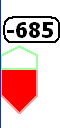
\includegraphics[angle=0,width=1.2cm,keepaspectratio='true']{figures/fig-finalglide-halfabove.png}}

In dieser Situation kann der Pilot entscheiden, ob er den Bart verlässt und den Endanflug
mit einer geringeren MC-Einstellung fortführt, oder er weitersteigen möchte.

Hier ist es sinnvoll, die Auto-MC Einstellung anzuschalten, die den MC-Wert automatisch auf den
optimalen MC-Wert einstellt. Hierdurch ist es extrem einfach für den Piloten, die ermittelte Steigrate
mit dem MC-Wert zu vergleichen. Wenn das erreichte Steigen unter das MC-Niveau fällt,
sollte der Bart verlassen werden

\item[\textit{Unter Endanflughöhe}]   bei MC$=M$, und etwas weniger als 500m  unterhalb bei MC$=0$
%\marginpar{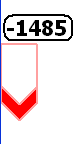
\includegraphics[angle=0,width=1.0cm,keepaspectratio='true']{figures/fig-finalglide-littlebelow.png}}
Das Display zeigt an, daß beim aktuellen MC-Wert die Endanflughöhe nicht erreicht ist,
bei MC$=0$, der jedoch nur weniger als 500m fehlen.
Mit dem gewählten MC-Wert fehlen satte 733m.
\marginpar{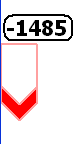
\includegraphics[angle=0,width=3.0em,keepaspectratio='true']{figures/fig-finalglide-littlebelow.png}}
\item[\textit{Unter Endanflughöhe}]  bei  MC$=M$, und bei MC$=0$

Die Aufgabe kann so nicht beendet werden, auch nicht bei MC$=0$.

\vspace{2em}
Das ist eine typische Anzeige zu Begin Einer Aufgabe, wenn man sich in Startnähe, oder aber noch noch am Boden befindet.  
Hier kann man sehr schön erkennen, wieviel man noch kurbeln muß.
\marginpar{
\includegraphics[angle=0,width=3.65em,keepaspectratio='true']{figures/fig-finalglide-allbelow.png}} 
%\marginpar{
\includegraphics[angle=0,width=1.0cm,keepaspectratio='true']{figures/fig-finalglide-allbelow.png}} 
\end{description}



Und hier mal ein Beispiel mit einer Komplettansicht der MovingMap:

\vspace{2em}
Hier hat man sich  verpokert. 


Die roten Pfeile zeigen, daß eine Außenlandung wahrscheinlich ist,  zu hoch gepokert \texttt{:-(}

Der Endanflug reicht weder mit dem eingestellten MC noch mit MC$=0$ aus, man erreicht weder den gewählten \sketch{figures/finalglide-allbelow.png}Wegpunkt \textsf{Damme}, dort gibt es deutlich vorher eine Geländekollision (gekennzeichnet durch das orange Kreuz auf der Karte), und der Ausweichflugplatz \textsf{Achmer} liegt gaaanz knapp außerhalb der Reichweite.

DG $\rightarrow$ Dumm Gelaufen \verb":-("

\vspace{2em}
\section{Ermittlung der Schnittgeschwindigkeiten}\label{sec:task-speed-estim}

Viele von \textsf{XCSoar's} internen Algorythmen benutzen Annahmen bzw.\ Vorhersagen für die Zeit, um
einen bestimmten Punkt zu erreichen. Dies sind Berechnungen ''in die Zukunft''  aus bisher 
gesammelten Informationen.

Diese Information wird in einigen Infoboxen benutzt, weiterhin auch in AAT-Aufgaben
sowie zur Warnung bei Erreichen nach Sonnenuntergang.

Der Rechner nimmt an, daß die erreichbare Überlandflug-Schnittgeschwindigkeit
gleich ist, wie die nach der klassischen MC-Theorie, Wind mit einberechnet.

Diese Annahme wird benutzt um Ankunftszeiten und Aufgabenankunft zu berechnen.

Die folgenden Aufgaben-Geschwindigkeiten sind definiert bzw. werden kalkuliert:
\begin{description}
\item[\textit{Bisher erreichte Aufgabengeschwindigkeit}]  Dies ist die \emph{aktuell
erreichte} Schnittgeschwindigkeit, kompensiert um die Höhe des Aufgabenstart 
%\todonum{was heißt das exakt? Wird die Höhe GND vom Startpunkt in pot.- Energie umgerechnet? $\frac{1}{2}\cdot m\cdot v^2 = m\cdot g\cdot h $  oder wie?}
\item[\textit{Mittlere Aufgabengeschwindigkeit}] Dies ist die angenommene
Schnittgeschwindigkeit, kompensiert um die Höhe, welche zur Beendigung der Aufgabe benötigt wird.
\item[\textit{Verbleibende Geschwindigkeit}]  Dies ist die angenommene Schnittgeschwindigkeit,
welche sich exakt nach der MC-Theorie ermittelt für den Task ergibt.
\item[\textit{Aktuelle Aufgabengeschwindigkeit}]  Dies ist der augenblickliche
angenommene Schnitt über die ganze Aufgabe
Wenn mit aktuell eingestelltem MC-Wert gekurbelt wird, ist dieser Wert
identisch mit der angenommenen Aufgabenschnittgeschwindigkeit.
Wenn in Bärten kleiner als der eingestellte MC-Wert gekurbelt wird, oder aber vom Kurs
abgewichen wird,  wird dieser Wert kleiner sein als die angenommene Schnittgeschwindigkeit.
Beim Vorfliegen in ruhiger Luft mit optimaler Geschwindigkeit wird diese Geschwindigkeit
gleich der angenommenen Aufgaben-Schnittgeschwindigkeit sein.

Dieser Wert, welcher als {\InfoBox} dargestellt werden kann, ist nützlich als eine kontinuierliche Anzeige
der Überlandperformance. Er wird nicht in anderen internen Kalkulationen zu Berechnungen herangezogen
\end{description}

Für AAT-Aufgaben wird anhand der MC-Einstellungen automatisch die optimale Position
der Wendepunkte errechnet.  \tip Wenn jeder Wendepunkt auf  'auto'  gesetzt wurde,  berechnet
\textsf{XCSoar} die Position der Wendepunkte derart, daß die AAT - Aufgabe nicht später als z.B. 5
Minuten nach der vorgegebenen Aufgabenzeit beendet wird.

Analog hierzu wird ein zusätzlicher MC-Wert '\emph{MC-erreicht}' {\em achieved MacCready} berechntet.
Dieser Wert wird so ermitteltt, indem vom erreichten Schnitt zurückgerechnet wird,
auf den MC-Wert, welcher dieselbe bisher erreichte Schnittgeschwindigkeit ergibt.

Der Wert ist größer als der aktuell eingestellte MC-Wert, wenn in stärkeren Bärten gekurbelt
wird, oder aber z.B. unter Wolkenstraßen geflogen wird.

Der 'MC-\emph{erreicht}' -Wert wird im Aufgaben-Dialog verwendet.

Die ermittelten Geschwindigkeitswerte für die bisher erreichten Schnitte sind höhenkompensiert,
sodaß Steigen und Sinken mit in die Ermittlung der mittleren Aufgaben-Schnittgeschwindigkeit eingehen:
Angenommen, zwei Flieger fliegen dieselbe Aufgabe.
Flieger A ist schneller vorgeflogen, verliert entsprechend Höhe für die Geschwindigkeit.
Flieger B ist hinter Flieger A, aber er ist höher und er wird Zeit sparen, da er weniger kurbeln muß, um
die Endanflughöhe zu erreichen.

Beim Fliegen von AAT Aufgaben können sich die Geschwindigkeitsangeban beim Einfliegen in
den Sektor ändern. Der Grund liegt darin,  daß evtl. der Pilot den Wendepunkt manuell
verschoben  oder den Sektor geändert hat. Da sich damit die zu fliegende Strecke ändert,
ändert sich zwangsläufig der Schnitt.


\section{Optimaler Vorflug-Kurs}

Um während des Vorfluges zwischen den einzelnen Wendepunkten (nicht im Endaflug!) den Weg-bzw.
Zeitverlust zu minimieren, wird \textsf{XCSoar} einen optimalen Weg, den "optimalen Vorflug-Kurs"
vorschlagen. Dieser Kurs ist optimiert, insofern als er die Windabdrift beim Geradeausflug als auch beim
Kurbeln mit einberechnet. Dementsprechend wird der MC-Wert ein anderer sein, als bei der klassischen
MC-Theorie.


\begin{center}
\begin{maxipage}
\centering
\def\svgwidth{0.8\linewidth}
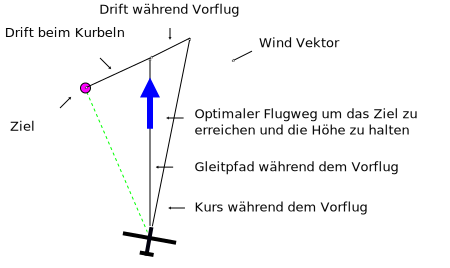
\includegraphics[angle=0,width=0.8\linewidth,keepaspectratio='true']{figures/figure_optimal_cruise-de.pdf}
\end{maxipage}
\end{center}

Der optimale Vorflugkurs wird als dicker blauer Pfeil auf dem Schirm angezeigt und er empfiehlt dem Piloten
exakt dieser Richtung nachzusteuern.

Wenn z.B. die Karte auf 'Kurs Oben'  (Track-Up) Anzeige eingestellt ist, steuere so, daß der dicke blaue Pfeil
genau nach oben zeigt.

Der optimale Kurs wird unter Berücksichtigung des Windes errechnet und zwar in der Art, daß sich die
schnellstmögliche Ankunft am Ziel ergibt. Wenn der Wind zu vernachlässigen ist oder sich der Rechner im
Endanflugmodus befindet, wird der blaue
Pfeil deckungsgleich mit der schwarzen Linie, die die Richtung zum nächsten Punkt angibt, sein.

Die Berechnung und Anzeige des optimalen Kurses ist einzigartig in \textsf{XCSoar}. Normalerweise,
wenn zwischen Bärten vorgeflogen wird, empfehlen Segelflugrechner, den Kurs direkt zum nächsten Wendepunkt.
Idealerweise aber sollten sie den Windversatz mit berücksichtigen, sodaß der minimale Weg zurückgelegt werden
muß, mit dem Nebeneffekt, schneller zu sein.

Sollte während des Endanfluges doch noch Kurbeln notwendig sein, so wird der Flieger auf jeden Fall
irgendwie versetzt, was der Rechner registriert und somit den track entsprechend anpaßt. Nach einigen
Bärten wird der Kurs daher eher kurvig bzw. zackig  angezeigt.

Für den Fall, daß das Ziel als Wegpunkt aktiv ist und man sich oberhalb der Endanflughöhe befindet, ist
ein Kurbeln nicht notwendig, daher ist dies einfache Schema optimal.

\section{Auto MacCready}\label{sec:auto-maccready}\index{MC-Optimierung}
\textsf{XCSoar} kann den MC-Wert automatisch anpassen, um den Piloten zu entlasten:
Dazu sind zwei Methoden bzw. Einstellungen möglich:
\begin{description}
\menulabel{\bmenut{Konfig.}{1/3}\blink\bmenut{MacCready}{Auto} }\item[\textit{Endanflug}]  
Während des Endanfluges wird der MC-Wert so optimiert, daß das Ziel in der
\emph{kürzest möglichen Zeit} erreicht wird.

Bei OLC-Sprint tasks wird der MC-Wert dagegen so angepaßt, daß \emph{eine
möglichst große Strecke} in der verbleibenden Zeit zurückgelegt wird und daß
das Ziel in der vorgegebenen Höhe erreicht wird!
\item[\textit{Erwartetes mittleres Steigen}]
Wenn man sich nicht im Endanflug befindet, wird der MC-Wert so gewählt, daß er dem
Mittelwert aller aller bisher erflogenen Bärte entspricht!
\item[\textit{Beides}] Zusätzlich können beide Methoden benutzt werden, sodaß vor
Erreichen des Endanfluges -also während der ganzen Aufgabe- das erwartete mittlere
Steigen herangezogen wird und im Endanflug optimiert auf die
 Ankunftszeit (streng nach MC-Theorie)  gerechnet wird.
\end{description}

(Zu deustch: einmal rechnet er besten Schnitt, einmal größte Strecke\dots im
dritten Falle kombiniert er beides )

%Ein- bzw. ausgeschaltet wird die Auto MC -Funktion mit
%\begin{quote}
%\bmenu{Konfig.}\blink\bmenut{Mac}{Auto}
%\end{quote}
In den Konfigurationseinstellungen ist  'Beides' als Standard voreingestellt.

Falls Auto MacCready angeschaltet wurde, erscheint 'AUTO'  in der MC-Infobox
anstelle von 'manuell'. Gleichzeitig erscheint in der Vario-Anzeige 'AutoMC' anstelle von 'MC'.

Diese Auto MC-Einstellungen werden hier hier im Anschluß beschrieben:

\subsection*{Endanflug}\index{Endanflug}
Wenn man sich über dem Gleitpfad befindet, so wird man in der Regel den MC-Wert etwas höher einstellen,
um schneller anzukommen. Indem man dies tut, setzt man automatisch voraus, daß die zu noch erwartenden
Bärte auch stärker werden.

Befindet man sich unterhalb des Gleitpfades, so wird man den MC-Wert etwas niedriger einstellen.
Damit nimmt man automatisch an, daß auch die Bärte entsprechend schlechter werden, in denen gekurbelt wird.

Die Funktion \textsl{Auto MacCready} nimmt diese Einstellung automatisch und kontinuierlich vor.
Normalerweise ist es sinnlos, diese Einstellung vor annähernd Erreichen der Endanflughöhe  zu wählen, da man sich
zu Begin des Fluges erheblich unterhalb der Endanflughöhe befindet und der Rechner mit dieser Einstellung dann
-logischerweise- den MC-Wert auf Null stellen würde.


\begin{maxipage}
\begin{center}
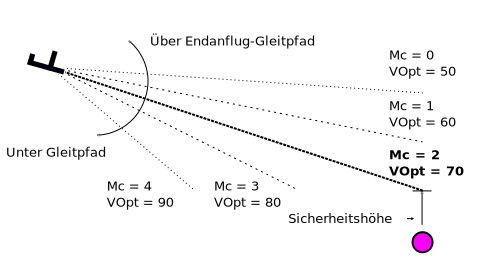
\includegraphics[angle=0,width=0.75\linewidth,keepaspectratio='true']{figures/figure_auto_maccready-de.pdf}
\end{center}
\end{maxipage}

\subsection*{Erwartetes mittleres Steigen}

Diese Einstellung stellt den MC-Wert auf den gemittelten Steigwert aller bisher erflogenen Bärte.
Damit wird automatisch auch die Zeit, welche in den Bärten verbracht wurde, berücksichtigt.
Der Wert wird nach jedem Verlassen eines Bartes aktualisiert.

Da die MC-Theorie genau dann optimal funktioniert, wenn der eingestellte MC-Wert exakt gleich dem
nächsten -leider unbekanntem- Bartsteigen, führt diese Theorie mitunter zu suboptimalen Ergebnissen,
z.B. Vorfluggeschwindigkeit zu langsam, falls sich die Bärte deutlich bessern, oder auch zu zu schnellem Vorflug,
falls sich die Wetterbedingungen verschlechtern.

Gleichzeitig,  falls der Pilot in über längere Zeit zu schwachem Steigen kurbelt,
wird dies das errechnete mittlere Steigern verringern, und so den Piloten veranlassen, auch
weiterhin in zu schwachen Bärten zu kurbeln.


\textsf{\textcolor[rgb]{0.00,0.00,0.50}
{Die genaue Kenntnis der Schwächen bzw. dieser Limitierungen
der MC-\textsl{Theorie} sollte  dem Piloten vertraut sein und ihn dazu veranlassen, sich mit dem
Gesamtsystem bestehend aus Wetter, Flugzeug, Piloten können und Software eingehend zu beschäftigen
und seine Entscheidungsfindung demgemäß zu treffen. Der Rechner/die Software allein kann nicht fliegen
und auch das Wetter nicht vorhersagen! Der Pilot kann wenigstens aus dem Cockpit schauen und eine
Regenfront erkennen!}}

\section{Analyse Dialog}\index{Analyse Dialog}

Der Analyse-Dialog kann z.B. dazu benutzt werden, um z.B. die Polare zu checken.
Die Funktion ist erreichbar über:

\menulabel{\bmenus{Info}\blink\bmenus{Analyse}}
%\begin{quote}
%\bmenu{Info}\blink\bmenu{Analyse}
%\end{quote}

Die Polare-Seite zeigt einen  Graphen der Polare mit den aktuellen Mücken und Ballast-Einstellungen.
Weiterhin ist das beste Gleiten und die dementsprechende Geschwindigkeit abzulesen, sowie das
minimale Sinken und die demenstprechende Geschwindigkeit.
Das vorher eingestellte  Startgewicht ist ebenfalls hier  abzulesen.

Mit \button{Einstellungen} wird die entsprechende Seite aufgerufen, auf der genau diese o.g.\ Werte geändert werden können.

\sketch{figures/analysis-glidepolar.png}
Die Flugzeugpolaren-Seite  des Analyse-Dialoges zeigt die totalenergiekompensierte Sinkrate bei der
entsprechenden Geschwindigkeit, wenn der Rechner mit einem intelligenten Vario verbunden ist.

Dies erlaubt es dem Piloten z.B. Testflüge in ruhiger Luft durchzuführen, um die Flugzeugpolare exakt zu vermessen.
Wird nun die gemessene \todonum{Wird hier wirklich die Polare aufgzeichnet?? 
Wird sie dann auch verwendet?  Wo wird sie dann abgespeichert?} mit der eingegebenen Polaren verglichen, erlaubt dies eine optimale Anpassung des Programmes an das jeweilige Flugzeug bei der jeweiligen Beladung und dies unter Berücksichtigung der optimalen Klappenstellung und anderen Optimierungsversuchen wie z-.B. Ruderspaltabdichtungen etc.

Die Daten werden ausschließlich erfaßt wenn die G-Rate zwischen 0,9 und 1,1 ist.
Man sollte also sehr ruhig fliegen, um die Aufzeichnungen nicht zu beeinflussen


%\begin{center}
%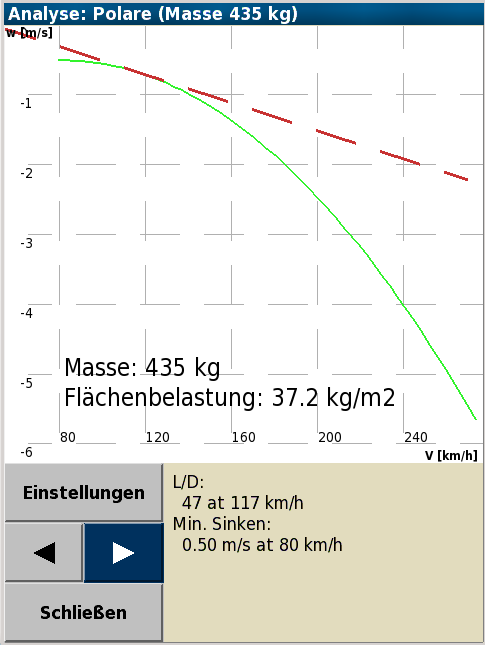
\includegraphics[angle=0,width=0.65\linewidth,keepaspectratio='true']{figures/analysis-glidepolar.png}
%\end{center}

\section{Hinweise zum Flug}\index{Hinweise zum Flug}\index{Meldungen während des Fluges}
Folgende Meldungen werden während des Fluges in einem
Meldefenster auf dem Bildschirm eingeblendet, wenn \xc errechnet, daß Zeiten bzw. Gleipfade nicht erreicht werden:

\begin{itemize}
\item[\textit{Erwarte frühe Aufgabenankunft}]  (bei AAT Aufgaben) Wenn die Aufgabe zu früh als gefordert beendet werden wird
\item[\textit{Erwarte Ankunft nach Sonnenuntergang}] Wenn die Aufgabe erst nach Sonnenuntergang beendet werden wird
\item[\textit{Erhebliche Windänderungen}] Wenn sich der Wind erheblich in Richtung oder Stärke geändert hat
\item[\textit{Über/unter dem Gleitpfad}]  Diese Meldung erscheint nur einmal bei Starten des Endanfluges, wenn sich das Flugzeug gemäß der \xc-Kalkulation über bzw.\ unter dem Gleitpfad auf das entsprechende Ziel befindet. 
Kann auch kontinuierlich während des gesamten Fluges an der linke Seite der Karte abgelesen werden, siehe Kap.\ref{sec:finalheight-indicator}
\end{itemize}
